%%%%%%%%%%%%%%%%%%%%%%% file template.tex %%%%%%%%%%%%%%%%%%%%%%%%%
%
% This is a template file for Web of Conferences Journal
%
% Copy it to a new file with a new name and use it as the basis
% for your article
%
%%%%%%%%%%%%%%%%%%%%%%%%%% EDP Science %%%%%%%%%%%%%%%%%%%%%%%%%%%%
%
%%%\documentclass[option]{webofc}
%%% "twocolumn" for typesetting an article in two columns format (default one column)
%
\documentclass{webofc}
\usepackage[varg]{txfonts}   % Web of Conferences font
\usepackage{listings}
\usepackage{xcolor}
\usepackage[colorlinks]{hyperref}
\usepackage{wrapfig}

\lstdefinelanguage{json}{
  string=[s]{"}{"},
  stringstyle=\color{blue},
  comment=[l]{:},
  commentstyle=\color{black}
}
\lstset{language=json}

\lstset { %
    belowcaptionskip=1\baselineskip,
    breaklines=true,
    % frame=L,
    xleftmargin=\parindent,
    language=C++,
    showstringspaces=false,
    basicstyle=\footnotesize\ttfamily,
    keywordstyle=\bfseries\color{green!40!black},
    commentstyle=\itshape\color{purple!40!black},
    identifierstyle=\color{blue},
    stringstyle=\color{orange},
    numbers=left
    % language=C++,
    % basicstyle=\ttfamily,
    % keywordstyle=\color{red}\ttfamily,
    % stringstyle=\color{gray}\ttfamily,
    % commentstyle=\color{blue}\ttfamily,
    % morecomment=[l][\color{magenta}]{\#}
    % backgroundcolor=\color{black!5}, % set backgroundcolor
    % basicstyle=\footnotesize,% basic font setting
    % numbers=left
}


%
% Put here some packages required or/and some personal commands
%
%
\begin{document}
%
\title{DQM4hep}
%
% subtitle is optional
%
\subtitle{A generic data quality monitoring framework for HEP}

\author{
\firstname{R\'emi} \lastname{Ete}\inst{1}\fnsep\thanks{\email{remi.ete@desy.de}}
\and
\firstname{Antoine} \lastname{Pingault}\inst{2}\fnsep\thanks{\email{antoine.pingault@ugent.be}}
}

\institute{
DESY, Notkestra\ss e 85, 22607 Hamburg, Germany
\and
Ghent University, Department of Physics and Astronomy Proeftuinstraat 86, B-9000 Gent, Belgium
}

\abstract{%
Data quality monitoring is the first step in the certification of data recorded for offline physics analyses.
Many experiments have developed their own dedicated monitoring system in the past.
Most of them rely on their own event data model (EDM), which leads to a strong dependency on the data format and storage.
We present here a generic data quality monitoring system, DQM4hep, that has been developed without any assumptions on the underlying event data model.
This reduces the code maintenance and increases the portability and reusability across other experiments.
We first introduce the framework architecture and the various core components as well as tools provided by the software package.
We give an overview of the different experiments using DQM4hep and the foreseen integration in future other experiments.
We finally present the ongoing and future software development for DQM4Hhep and long-term prospects.
}
%
\maketitle
%
\section{Introduction}
\label{sec:intro}

Online data quality monitoring systems are crucial while taking experimental data.
The main tasks of such tools are to provide a quick overview of the detector and sub-detector status and to evaluate the quality of these data.
More technically, the online framework should provide the following ingredients:

\begin{itemize}
  \item a link to the data acquisition system (DAQ) to access the detector data and run control status.
  \item a dedicated online analysis and data quality assessment framework.
  \item a visualization system to show the resulting analysis products.
\end{itemize}

Such systems are generally (but not always) decoupled from the data quality monitoring done offline on recorded data or simulated data.
Often, the architecture of these software relies on the event data model (EDM) of the underlying experiment. This can be seen as a limitation, as the software becomes non-reusable by other experiments.

In this paper, we present a new generic framework for online and offline data quality monitoring called DQM4hep.
After introducing the framework architecture and specifications, the different components of DQM4hep are described.
The software still being in development, we conclude with a few perspective and incoming features.

\section{The DQM4hep framework}
\label{sec:framework}

\subsection{Software architecture and specifications}
\label{subsec:arch}

The DQM4hep framework is built on top of the so-called plugin system component.
A plugin is a C++ class encapsulating a user class that is compiled in a shared library and loaded at runtime by the plugin system.
The plugin is used as a factory to create instances of the user class on demand.
Such a system allows for building a framework with which the behavior of the key components can be changed at runtime.

In order to have a really generic monitoring system, the software should not depend on any EDM or data format.
This allows having highly-reusable software for different experiments.
By construction, in DQM4hep, the data type is user-defined and wrapped in a higher level handler (\texttt{dqm4hep::Event}).
As the data has to be transported over the network, the data streaming, file reading and writing facilities, have to be user-defined.
The user-streaming interface can be encapsulated in a plugin that the framework can use in online applications to serialize (de-serialize) data before sending (after receiving) to (from) an endpoint.

\begin{figure}[!h]
  \centering
  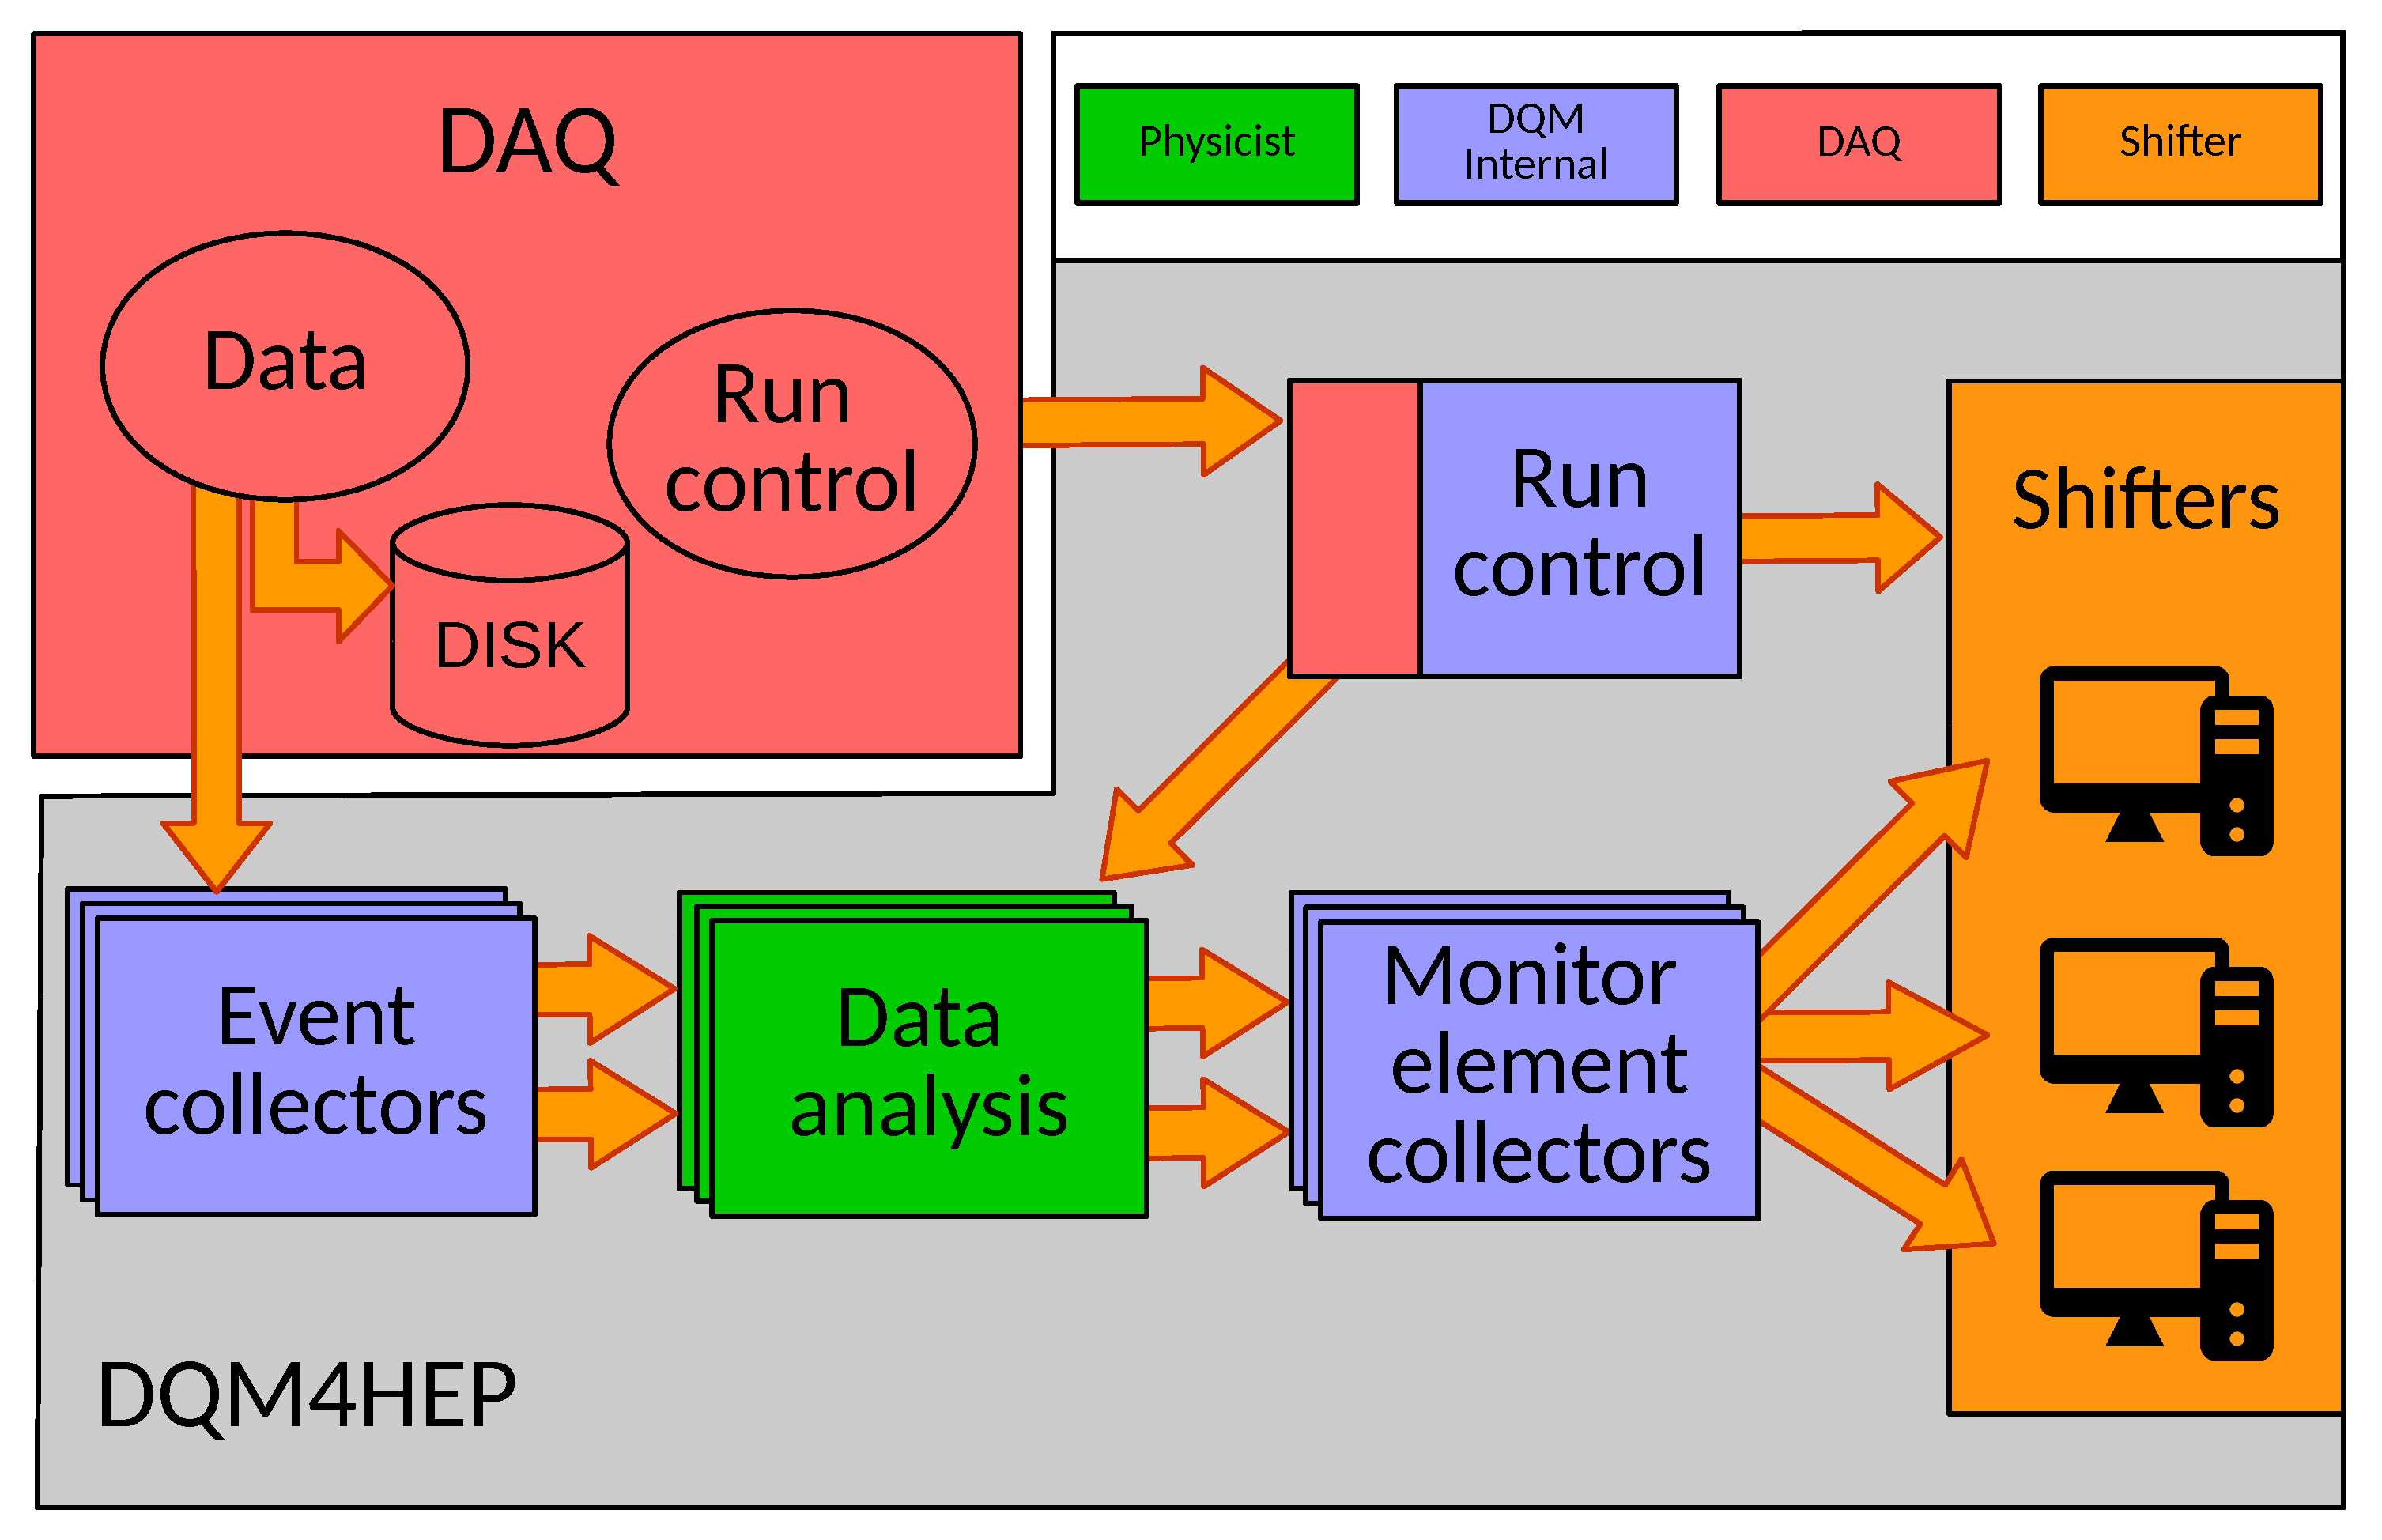
\includegraphics[width=.95\textwidth]{figs/AnalysisModuleArchitecture.pdf}
  \caption{Online architecture of the DQM4hep framework. The top left corner corresponds to the DAQ system and is not part
  of the framework, it is displayed here to show the link between the two systems.}
  \label{fig:GlobalArchitectureDiagram}
\end{figure}

An important requirement for the online component of the monitoring system is to be distributed.
A typical user analysis handles tens or hundreds of histograms that are filled whenever data are received from the DAQ system.
The analysis program, in this case, is particularly \textit{greedy} in terms of memory.
Analyzing data in a single process is thus very limited and must be distributed over different processes or computers depending on the available resources on each machine.
This also increases the speedup of analysis as the resources are shared and allows for more data to be processed in the same amount of time.
The online analyses applications have to be carefully designed in terms of memory management as they may run for many hours and must stay stable.

Before analyzing them, data needs to be forwarded from the DAQ system to the monitoring system.
The mechanism may be of many forms: shared-memory (if running on same computers), network (TCP/IP), database, etc. but a major requirement is to avoid slowing or crashing the acquisition process.
A global overview of the framework's online architecture is shown in~\autoref{fig:GlobalArchitectureDiagram}.

\subsection{The core components}
\label{subsec:core}

\paragraph{The plugin system}

As stated before, DQM4hep is built on top of a plugin system.
The \texttt{dqm4hep::PluginManager} class is a singleton class holding all plugins within an application.
The plugins are loaded by opening shared libraries using the \texttt{::dlopen()} function at startup.
A user class object can be created on the heap by querying a specific plugin to the \texttt{dqm4hep::PluginManager} and
by calling \texttt{dqm4hep::Plugin::create()}.

\paragraph{The event data model}

The core component of DQM4hep defines a high level handler, \texttt{dqm4hep::Event}, wrapping a user-defined event class.
This handler is particularly useful because it allows to transport the user-defined event through an application
workflow without making any assumption on the underlying implementation:

\begin{lstlisting}{language=C++}
// a user defined function
dqm4hep::EventPtr createEvent() {
  // a DQM4hep event ...
  dqm4hep::EventPtr event = dqm4hep::Event::create<MyEvent>();
  // ... wrapping a user-defined structure
  MyEvent *myevt = event->get<MyEvent>();
  myevt->setTimeStamp(time(0));
  myevt->setData({0.5, 856., 485.});
  return event;
}
\end{lstlisting}

\paragraph{Event streaming}

To send (receive) events to (from) the network, events have to be converted from or to a format that the transport system can handle (e.g binary).
As the event is user-defined, the event streaming also has to be user-defined.
The framework defines a base class \texttt{dqm4hep::EventStreamerPlugin} to stream in and out events that users have to implement:

\begin{lstlisting}{language=C++}
class EventStreamerPlugin {
public:
  // creates user-defined event
  virtual EventPtr createEvent() const = 0;
  // write event to TBuffer object
  virtual StatusCode write(EventPtr event, TBuffer &buffer) = 0;
  // read event from TBuffer object
  virtual StatusCode read(EventPtr event, TBuffer &buffer) = 0;
};
\end{lstlisting}

The streamer implementation can be declared as a plugin and loaded at runtime using the \texttt{dqm4hep::PluginManager}.
The combination of \texttt{dqm4hep::PluginManager}, \texttt{dqm4hep::Event} and \texttt{dqm4hep::EventStreamerPlugin} gives the fully required flexibility for such a framework.

{ % bracket needed for wrapfigure for this paper ...

\begin{wrapfigure}{R}{0.5\textwidth}
    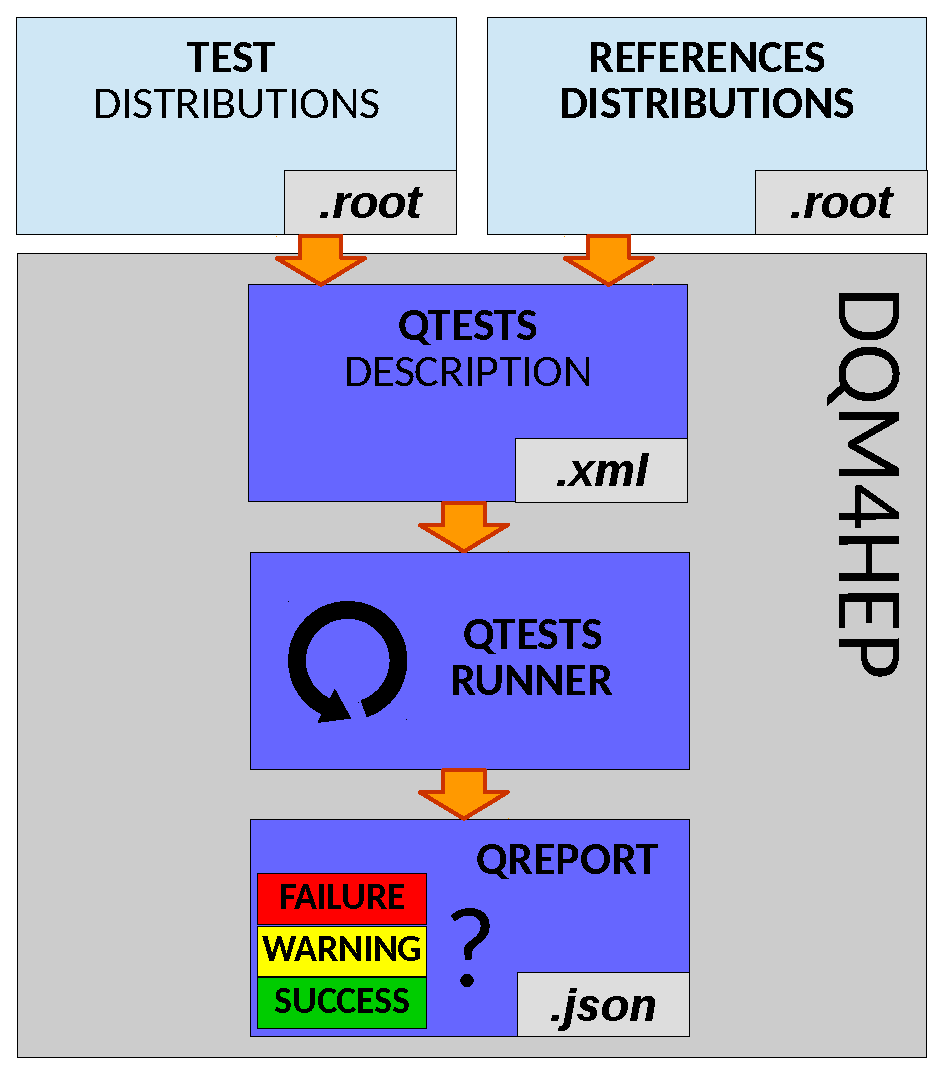
\includegraphics[width=\linewidth]{figs/QTestRunner.pdf}
    \caption{Offline quality test processing workflow: from monitor elements and references to quality test reports.}
    \label{fig:QTestsAndQReports}
\end{wrapfigure}

\paragraph{Monitor elements}

The concept of \textit{monitor element} is central in data quality monitoring software.
It encapsulates a summary of the data being monitored by the framework.
One dimension histograms are the most commonly used monitor element types in HEP, but it can also be scalar values (counters), time-stamped graphs (environmental variables), 2D histograms (hit maps), etc.

\paragraph{Quality test and report}

Whereas the monitor element provides a summary of a data set, the \textit{quality test} implements the logic of testing an element or evaluating its quality.
These tests are also designed to detect problems as some observables (mean of distributions, counters, etc.) may deviate from expectations during or after data taking. \autoref{fig:QTestsAndQReports} shows the workflow of monitor elements

} % bracket needed for wrapfigure for this paper ...
% infortunately have to do the job of wrapfigure here ...
\noindent testing in offline mode.
Monitor elements are stored as \texttt{ROOT}~\cite{ROOT} objects with potential reference entities provided by experts.
Monitor elements can thus be compared to the references as part of a quality test or at a later stage by an operator.
The quality tests and the monitor elements to test are described in XML format and passed to a program for processing.
A \textit{quality test report}, containing quality test status (success, warning, failure), quality estimate (in the range [0;1]) and additional custom user data, is output in JSON format.

\subsection{The online system}
\label{subsec:online}
The main purpose of a data quality monitoring system is the visualization and quality assessment of detectors data in a real-time environment.

\paragraph{Collectors}\label{par:Collectors}
The first stage in achieving this objective is the transmission of the data from the DAQ system to the analyses modules.
This is done by building and wrapping user-defined event from the DAQ data as DQM4hep events before streaming them to the analyses modules.
Since there might be an indefinite number of modules running on multiple hosts, there is a need for a central access and distribution point of this data. This is the role of the collectors, of which two types are defined:

\begin{itemize}
  \item The \textit{event collector}, which collects \texttt{dqm4hep::Event} from the event builder and distributes them to the analyses modules.
  \item The \textit{monitor element collector}, which collects the products of these analyses, the \textit{monitor elements}, and distributes them to the visualization interfaces.
\end{itemize}

\paragraph{Modules}\label{par:Modules}
Two major data flavors are needed when running an experiment, the physics data from the detector itself and the data from the slow control systems.
To cope with these two possible kinds of input, two types of modules are defined within the framework: the analysis module and the standalone module.
They are both user-defined plugins that can be started or stopped at any point while the framework is running.
Their goal is to reduce the initial amount of data to a few useful elements, the \textit{monitor elements}.
Quality tests can assess the output data and resulting quality test reports stored within the \textit{monitor element} and sent along to the \textit{monitor element collectors}.

Where analyses modules use DQM4hep event streamed by the \texttt{event collectors} as input, the standalone modules use data from external sources (pressure sensors, detector high voltages, etc.).
These external sources, and thus the modules, operate independently of the DAQ system.
A standalone module can include some analysis but is most of the time just used to process the raw external data for visualization and data quality assessment.
Analyses modules can be run independently in online or offline mode.
In this context, offline means there is no detector system running, and no operator is waiting for the data to be displayed continuously.
There is thus no incentive to process and display the data in real time: the data is read and stored from and to disk, and no run management is needed.
This mode is especially useful for quality assessment of simulation data and new analyses testing.

\subsection{The online visualization}
\label{subsec:vis}

To ease the use of the framework, several Graphical User Interfaces (GUI) were implemented.
For now, only QT~\cite{QT} based interfaces are fully functional and available for end-users.

\paragraph{Job control}\label{par:JobControl}

The framework needs multiple applications (jobs) to run at the same time (collectors, modules, run control server, etc.), sometimes over different host for load balancing purposes.
For practical reasons, it is important to easily control and monitor these processes from a central point.
This is achieved through the use of \textit{Job control servers} that run as daemons on every host taking part in the deployment.
They wait for remote client interfaces, called \textit{Job control interfaces}, to connect and manage the local processes.
A GUI, the \textit{job control interface}, is used as a central point to monitor and control all the jobs across all the hosts.
When using this interface, all the jobs needing to run have to be defined and configured (process name, host, options, etc.) through a JSON configuration file.
To simplify this configuration process, the framework implements a JSON parser which extends the default JSON functionalities such as comments and variable expansion.

\paragraph{Main Monitoring Window}\label{par:MainGUI}

Most users will predominantly use only this interface as its function is to display the end results of the analyses and quickly give an overview of the quality of the data being taken.
A general view of this interface can be seen in~\autoref{fig:DQMMainViz}.
The first step in using this interface consists to browse the available \texttt{Monitor Element Collectors} and select the \texttt{Monitor Elements} of interests.
This is done through the \textit{browse} window which provides various search function (by ME name, module, etc.) to help construct this selection.
A tree-like structure, with folders and sub-folders, is then available on the left side of the main interface to navigate previously selected ME.
Apart from the top-level folders, which are named after the analysis module the ME belongs to, the organization of this structure is user-defined within each module.
The user can then select which \texttt{ME} to display in the drawing area.
Once displayed, they can be rearranged at will within the drawing area and multiple tabs can be opened to show different subsets of interesting \texttt{ME}.
The window background (\textcolor{red}{\textbf{Or is it only the small icon on the top left corner?}}) of each \texttt{ME} is colored depending on the results of its selected quality test for a quick visual assessment of its quality from the user.
Multiple tests can be assigned to each \texttt{ME} and their details and report can be accessed via a context menu. \textcolor{red}{\textbf{What happens to the icon color when multiple tests are defined? I suppose only one of them is used?}}
As mentioned before each \texttt{ME} is a valid ROOT object and can, therefore, use all the functionalities ROOT offers (fitting, re-scaling, etc.).
This proves particularly useful during data taking to quickly glance and analyze a specific subset of data.
Multiple instances of this interface can be opened on any host, provided they are on the same network and connect to the available \textit{Monitor Element Collectors}.

\begin{figure}
  \centering
  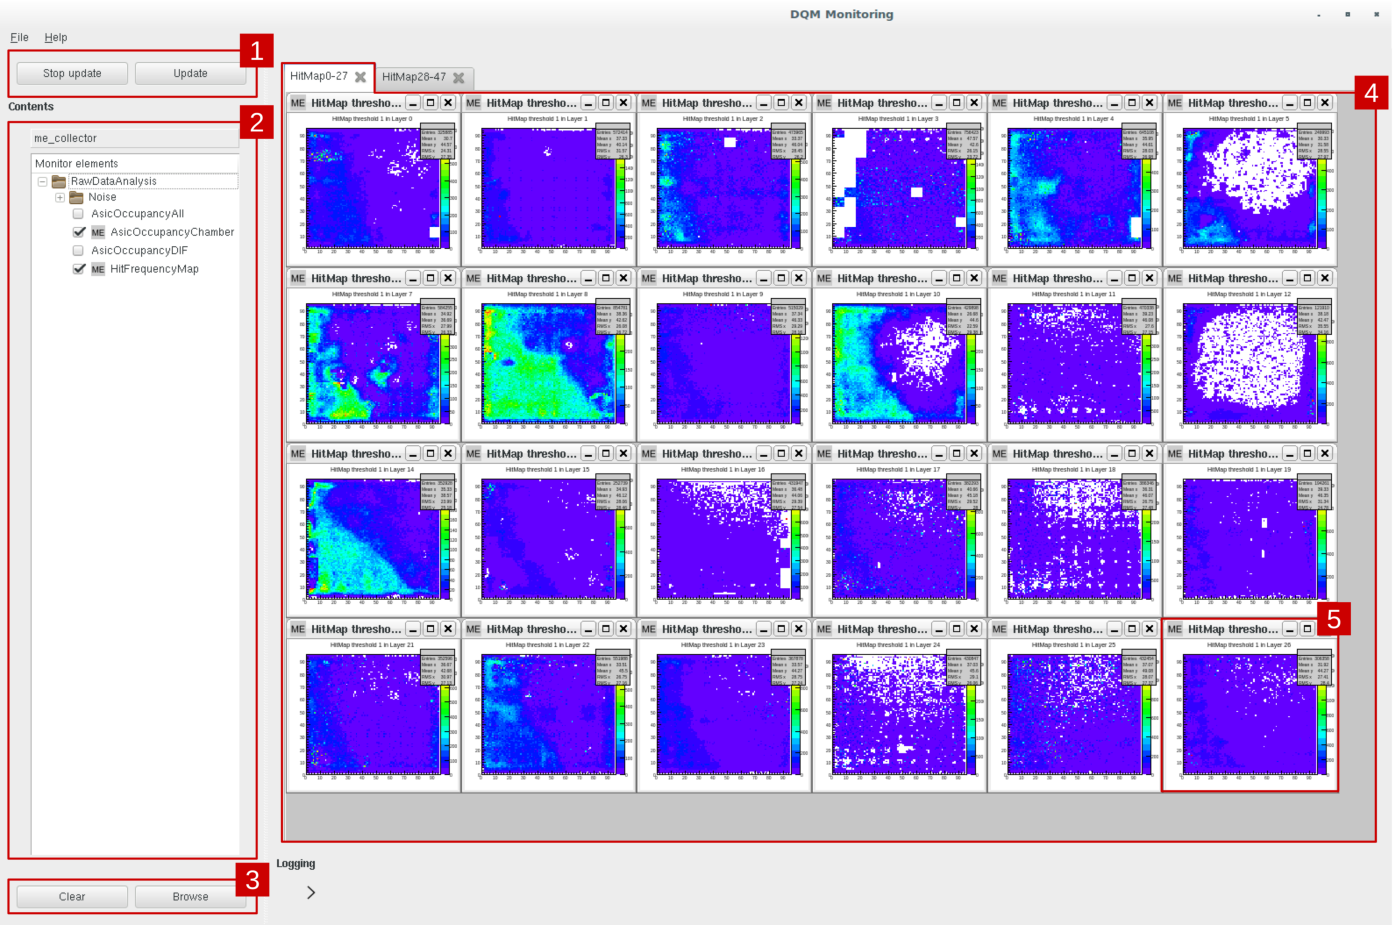
\includegraphics[width=.95\textwidth]{figs/MaintInterfaceGUI.pdf}
    \caption{\label{fig:DQMMainViz} Main window of the monitoring GUI.
    1: Option for manual/auto update.
    2: \texttt{Monitor Elements} (\texttt{ME}) organized in a tree-like structure
    3: Open Browse window to create \texttt{ME} selection available in 2.
    4: Drawing section for \texttt{ME}, can be organized in multiple tabs.
    5: Drawn \texttt{ME} are valid ROOT object that can be manipulated (zoom, scale change, fit, etc.)
    }
\end{figure}

\paragraph{Web Interface}\label{par:WebGUI}
A web-based interface regrouping all the GUI mentioned has also been developed. As of this writing, it is still missing some key links to the back-end to be fully operational for the end-users. The main advantage of such interface is the portability as the only prerequisite is a recent internet browser.

\section{Detectors using DQM4hep}
\label{sec:detectors}

The work on this framework was started within the CALICE~\footnote{CAlorimeter for LInear Collider Experiment}-Semi Digital Hadronic CALorimeter (SDHCAL) collaboration.
As such, a dedicated implementation, based on the LCIO~\cite{LCIO} Event Data Model and including multiple analyses modules, was produced to demonstrate the capabilities of the framework.
For the past three years and five test beam campaigns, the SDHCAL prototype successfully used this tool as their online data quality monitoring (DQM) system.

Since then, other experiments from the CALICE collaboration adopted the framework for their DQM needs. It has also been deployed for a combination of two separate detectors using different data acquisition systems, demonstrating the reusability and scalability of the system.


\section{Conclusion}
\label{sec:conclusion}

A new generic framework for data quality monitoring for high energy physics, DQM4hep, has been developed without any assumption on the underlying event data model implementation or data format.
These core \textcolor{red}{\textbf{guidelines (find better phrasing)}} promote high degrees of portability and reusability across experiments.
This software solution provides tools to develop data analyses and quality assessment of any experiments data.
It can be deployed for both online (i.e real-time data taking) and offline (i.e simulation or pre-recorded data) setups.

Visualization interfaces have been developed with Qt4 libraries for steering the online deployment and displaying the monitor elements collected during data taking.
The framework has now been used in real-world condition by several detector prototypes across multiple test beam campaigns for their monitoring needs, \textcolor{red}{\textbf{showing the reusability of the solution. (meh)}}
For some of these campaigns, the data acquisition was performed with multiple sub-detectors, and the framework deployed across several computers, demonstrating the scalability of the software.

Web tools are currently in development to replace the GUI tools and improve the portability of user interfaces.

% BibTeX or Biber users please use (the style is already called in the class, ensure that the "woc.bst" style is in your local directory)
\bibliography{dqm4hep}

\end{document}
